\section{Projekta apraksts}

    Tika izveidota \texttt{Blazor Server} tīmekļa aplikācija, izmantojot \texttt{Blazor} ietvaru, kur lietotājs
    ar pelītes palīdzību var uzzīmēt, piemēram, kādu ciparu, un tika izveidots mašīnmācīšanās modelis,
    izmantojot \texttt{MNIST} datu kopu, kas analizē uzzīmēto ciparu un atgriež procentuālu sadalījumu
    ar datu kopas klasēm. Klase ar augstāko rezultātu paredz uzzīmēto ciparu. Tā kā projekts ir apjomīgs,
    tas tika veikts grupā. Projekts tika sadalīts divās daļās - tīmekļa aplikācijas izstrāde un
    mašīnmācīšanās modeļa izstrāde. Attiecīgi autori izvēlējās darbu sadalīt:

    \begin{itemize}
        \item Arina Solovjova atbildīga par uzdevumiem saistībā ar tīmekļa
    aplikācijas izstrādi
        \item Kristofers Volkovs atbildīgs par mašīnmācīšanās modeļa izstrādi.
    \end{itemize}

    % Description about the created web page
    \subsection{Tīmekļa aplikācija}
Tīmekļa aplikācijas lapas sastāvā galvenie elementi ir zīmēšanas \texttt{canvas}, uz kura lietotājs var zīmēt izvēlēto ciparu. Tas sastāv no \texttt{svg} elementa, kurš uztur vairākus \texttt{polyline} elementus. Elementam ir piesaistītas tādas funkcijas, kā zīmējuma pilnīga izdzēšana, pēdējās darbības atcelšana, iespēja lejupielādēt uzzīmēto attēlu un iespēja padot zīmējumu mašīnmācīšanās algoritmam, lai tas analizētu uzzīmēto.
\par Zīmējuma izdzēšanas funkcija ir pievienota pie pogas 'CLEAR'. Funkcija izdzēš visus uz zīmēšanas \texttt{canvas} uzzīmētos \texttt{polyline} elementus, kas ir saglabāti. Funkcija, kas tiek izsaukta ar pogu 'UNDO', izdzēš pēdējo uz zīmēšanas \texttt{canvas} uzzīmēto \texttt{polyline} elementu. Poga 'GUESS' izsauc funkciju, kas padod uzzīmēto ciparu mašīnmācīšanās algoritmam. Poga'SAVE' izsauc funkciju, kas saglabā uzzīmēto lietotāja datorā.
\par Ir papildus pievienota zīmējumu un minējumu vēsture. Zīmējumi tiek attēloti samazinātā formātā ar mašīnmācīšanās algoritma rezultātiem. Zīmējumu vēstures elementus ir iespējams izdzēst, atsevišķi atlasot noteikto zīmējumu un uzspiežot uz pogas 'DELETE'. Poga izsauc funkciju, kas izdzēš noteikto elementu no saglabāto zīmējumu saraksta.


    % Description about the created ML model
    \subsection{Mašīnmācīšanās modelis}

    Mašīnmācīšanās modeļa izstrādi ir iespējams sadalīt vēl divās daļās: modeļa trenēšana un modeļa
    implementācija tīmekļa aplikācijā.

    Sākotnēji tika veikta izpēte par to, kādi gatavi
    ietvari jau eksistē \texttt{C\#} ekosistēmā. Tika atrasti tādi ietvari, kā \texttt{PyTorch.NET},
    \texttt{Keras.NET}, \texttt{ML.NET} un \texttt{CNTK}. Sākumā bija plānots izmantot \texttt{CNTK},
    bet izpētes processā tika secināts, ka Microsoft ir pārtraukuši atbalstu \texttt{CNTK} un vairs
    to neuzlabos un neatjaunos \cite{chrisbasogluCNTKReleaseNotes}. Šī iemesla dēļ netika izmantots
    \texttt{CNTK} ietvars. Ņēmot vērā tādus faktorus kā laiku un darba autora pieredzi tika izvēlēts
    \texttt{ML.NET} ietvars. Citi ietvari netika izmantoti, jo modeļa izstrāde ar tiem aizņemtu
    daudz vairāk laika, tapēc būtu iespēja, ka darbs netiktu pabeigts laikā.

    Attiecīgi tika izveidota programma, kas apmāca modeli, izmantojot \texttt{MNIST} datu kopu, un
    šīs programmas darbība ir aprakstīta \ref{ml:train}~attēlā. Kā piemēri tika izmantoti citi jau
    eksistējoši \texttt{GithHub} projekti un \texttt{ML.NET} un \texttt{MNIST} dokumentācija.
    \cite{DotnetMachinelearningsamples2021} \cite{kexugitTestRunWorking} \cite{MLNETTutorial}
    \cite{natkeMLNETDocumentation} \cite{paxbunPaxbunCntkMnistPractice2019}

    \begin{figure}[H]
        \centering
        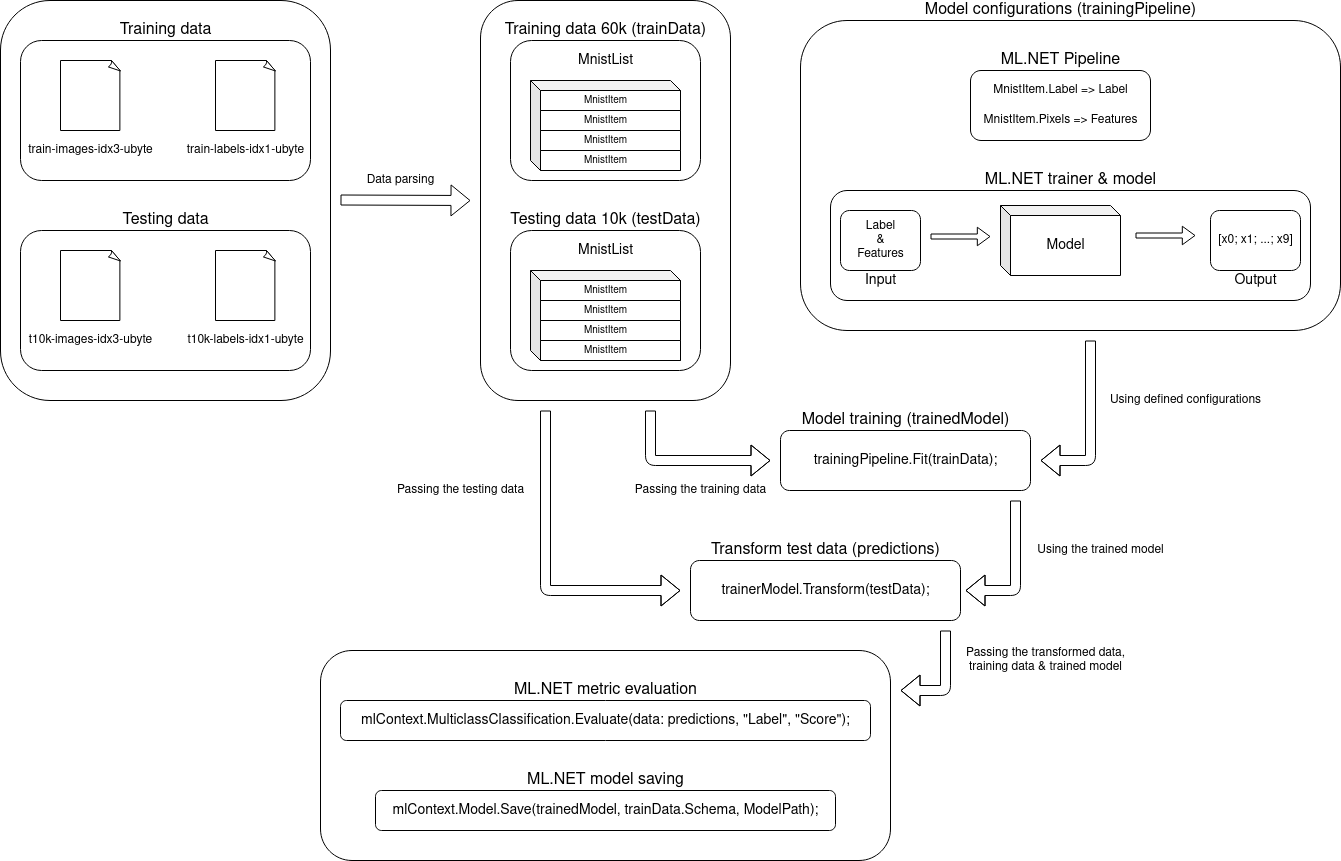
\includegraphics[width=15cm]{VPL-ML.png}
        \caption{ML modeļa trenēšanas diagramma}
        \label{ml:train}
    \end{figure}

    Projekta sākumā tika iegūti \texttt{MNIST} dati no "THE MNIST DATABASE". Tie ir 4 bināri faili
    un tos diagrammā var redzēt "Training data" un "Testing data" kvadrātos. Pēc datu iegūšanas tika
    izveidots datu parsēšanas funkcija, kas ielasa visus datus atmiņā un sadala tos pa klasēm
    \texttt{MnistList} un \texttt{MnistItem}. Šīm klasēm ir arī vizuāla reprezentācija diagrammā.
    Kad dati ir ielādēti atmiņā, tad tiek izveidots \texttt{ML.NET} "pipeline", kas ir kā konfigurācija
    priekš modeļa, kas tiks apmācīts. Visa konfigurācija ir redzama "Model configurations" kvadrātā. Šajā konfigurācijā
    tiek izveidots "pipeline", kas sasaista \texttt{Mnist} klašu mainīgos ar modeļa mainīgajiem.
    Tiek arī nodefinēta modeļa veids, kādi input dati būs un kādi output dati. Pēc datu ielasīšanas
    un modeļa nokofigurēšanas šis modelis tiek apmācīts. Lai šo modeli apmācītu, tiek izmantotas
    \texttt{ML.NET} iebūvētā metode: \texttt{.Fit()}. Šo funkcijju ir iespējams apskatīt "Model training"
    kvadrātā. Kad modelis ir apmācīts ir nepieciešams novērtēt cik labi šis modelis ir apmācīts, tapēc
    ir nepieciešams veikt transformācijas uz testa datiem tas ir redzams "Transform test data" kvadrātā,
    un tad, izmantojot šos pārveidotos testa datus, un \texttt{ML.NET} iebūvēto funkciju \texttt{.Evaluate()}
    tiek iegūtas modeļa rezultējošās metrikas. Pēdējais solis ir šo modeli saglabāt, kas arī tiek darīts
    izmantojot \texttt{ML.NET} iebūvēto funkciju \texttt{.Save()}.

    Rezultātā tika iegūts modelis, kuru metriku rezultāti ir redzami \ref{ml:metrics}~attēlā.

    \begin{figure}[H]
        \centering
        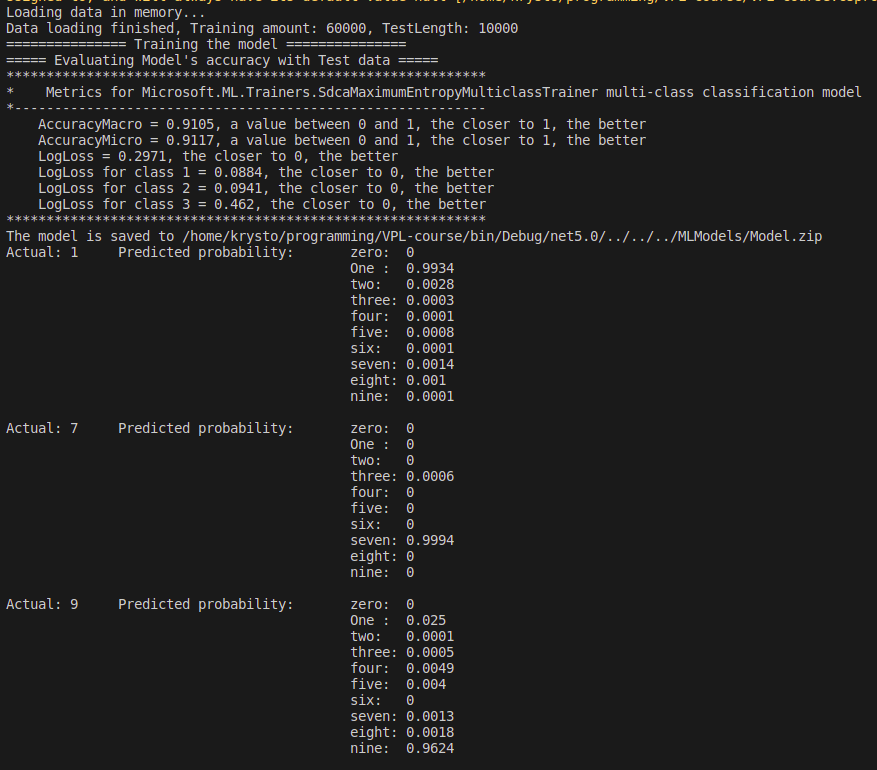
\includegraphics[width=13cm]{training-sc-v2.png}
        \caption{ML modeļa metriku rezultāti}
        \label{ml:metrics}
    \end{figure}

    Kad modelis bija izveidots, tad to bija nepieciešams implementēt tīmekļa aplikācijā. Tika izveidota
    \texttt{MnistClassificator} klase, kurā atrodas  metode \mintinline{csharp}{public float[] Analyze(byte[] image)}, kas tiek padota izveidotam modelim, kas atgriež
    virkni ar float vērtībām. Šīs vērtības reprezentē procentuālās vērtības ciparu klasēm.

